% !TEX root =  ../pers_schedules.tex 
\section{Simulation study}

\subsection{Results with $\kappa$ chosen on the basis of Youden's J}
In the main manuscript, for the personalized schedules based on dynamic risk of GR we chose $\kappa$ on the basis of $F_1$ score. However while conducting the simulation study, we also tried choosing it on the basis of Youden's $J$. Unlike $F_1$ score, Youden's $J$, is a measure of classification accuracy for both cases and controls. It is defined as:
\begin{align*}
J(t, \Delta t, s) &= \text{TPR}(t, \Delta t, s) - \text{FPR}(t, \Delta t, s), J\epsilon [-1,1],\\
\text{TPR}(t, \Delta t, s) &= \mbox{Pr}\big\{\pi_j(t + \Delta t \mid t,s) \leq \kappa \mid T^*_j \epsilon (t, t + \Delta t]\big\},\\
\text{FPR}(t, \Delta t, s) &= \mbox{Pr}\big\{\pi_j(t + \Delta t \mid t,s) > \kappa \mid T^*_j > t + \Delta t \big\}
\end{align*}
where $\mbox{TPR}(\cdot)$ and $\mbox{FPR}(\cdot)$ denote time dependent true positive rate (sensitivity) and false positive rate ($1 - \mbox{Specificity}$). The estimation for both proceeds as in \citep{rizopoulosJMbayes}. The optimal value of $\kappa$ is $\argmax_{\kappa} J(t, \Delta t, s)$.

The simulation study results for Youden's $J$ were not presented in the main manuscript for brevity and are presented here in Web Table \ref{table : sim_study_pooled_estimates_extended}. In addition results for a hybrid approach between median time of GR and dynamic risk of GR based on Youden's $J$ are also presented.

\begin{table}[!htb]
\caption{Estimated mean and standard deviation of the number of biopsies and offset (months). Method names are abbreviated for consistency with Figure \ref{fig : meanNbVsOffset}.}
\label{table : sim_study_pooled_estimates_extended}
\begin{tabular}{lrrrr}
\Hline
\multicolumn{5}{c}{a) All subgroups: 101823 patients}\\
\hline
Schedule          & $E[N^{bS}]$ & $E[O^{S}]$ & ${\mbox{SD}[N^{bS}]}$ & ${\mbox{SD}[O^S]}$ \\
\hline
Annual         & 5.24            & 6.01                & 2.53          & 3.45              \\
PRIAS          & 4.86            & 8.49                & 2.35          & 8.69\\
Exp. GR time & 1.92            & 15.06               & 1.19          & 12.11             \\
Med. GR time & 2.07            & 13.87               & 1.42          & 11.80              \\
Dyn. risk GR ($F_1$ score)       & 4.69            & 6.66                & 2.20           & 4.37              \\
Mixed ($F_1$ score)       & 3.75            & 9.69                & 1.71          & 7.02              \\
Dyn. risk GR (Youden's $J$)      & 4.56            & 8.04                & 2.00             & 11.08 \\
Mixed (Youden's $J$)   & 3.76            & 9.78                & 1.70           & 7.71    \\
\hline
\multicolumn{5}{c}{b) Subgroup $G_1$: 33680 patients}\\
\hline
Schedule        & $E[N^{bS}]$ & $E[O^{S}]$ & ${\mbox{SD}[N^{bS}]}$ & ${\mbox{SD}[O^S]}$ \\
\hline
Annual         & 4.33            & 6.02                & 3.14          & 3.44              \\
PRIAS          & 4.05            & 7.98                & 2.87          & 8.08     \\
Exp. GR time & 1.72            & 21.65               & 1.47          & 14.77             \\
Med. GR time & 1.85            & 20.67               & 1.77          & 14.64             \\
Dyn. risk GR ($F_1$ score)       & 3.85            & 6.76                & 2.69          & 4.45              \\
Mixed ($F_1$ score)       & 3.24            & 10.24               & 2.17          & 7.73              \\
Dyn. risk GR (Youden's $J$)      & 3.73            & 9.02                & 2.41          & 14.78            \\
Mixed (Youden's $J$)   & 3.26            & 10.4                & 2.16          & 8.80               \\
\hline      
\multicolumn{5}{c}{c) Subgroup $G_2$: 33907 patients}\\
\hline
Schedule        & $E[N^{bS}]$ & $E[O^{S}]$ & ${\mbox{SD}[N^{bS}]}$ & ${\mbox{SD}[O^S]}$ \\
\hline
Annual         & 5.18            & 5.99                & 2.13          & 3.48              \\
PRIAS          & 4.82            & 8.57                & 1.99          & 8.65        \\
Exp. GR time & 1.78            & 13.53               & 0.98          & 9.82              \\
Med. GR time & 1.90             & 12.31               & 1.16          & 9.43              \\
Dyn. risk GR ($F_1$ score)       & 4.63            & 6.66                & 1.82          & 4.34              \\
Mixed ($F_1$ score)       & 3.68            & 10.30                & 1.38          & 7.17              \\
Dyn. risk GR (Youden's $J$)      & 4.52            & 7.67                & 1.67          & 9.42           \\
Mixed (Youden's $J$)   & 3.70             & 10.42               & 1.36          & 7.77              \\
\hline      
\multicolumn{5}{c}{d) Subgroup $G_3$: 34236 patients}\\
\hline
Schedule        & $E[N^{bS}]$ & $E[O^{S}]$ & ${\mbox{SD}[N^{bS}]}$ & ${\mbox{SD}[O^S]}$ \\
\hline
Annual         & 6.20             & 6.01                & 1.77          & 3.46              \\
PRIAS          & 5.70             & 8.92                & 1.73          & 9.27        \\
Exp. GR time & 2.27            & 10.11               & 0.99          & 7.53              \\
Med. GR time & 2.45            & 8.71                & 1.15          & 6.36              \\
Dyn. risk GR ($F_1$ score)       & 5.57            & 6.58                & 1.56          & 4.32              \\
Mixed ($F_1$ score)       & 4.31            & 8.54                & 1.27          & 5.91              \\
Dyn. risk GR (Youden's $J$)      & 5.42            & 7.45                & 1.44          & 7.81  \\        
Mixed (Youden's $J$)   & 4.32            & 8.55                & 1.25          & 6.19              \\
\hline     
\end{tabular}
\end{table}

\subsection{Plots for the results of simulation study}
In this section we present figures related to the simulation study results discussed in Section \ref{sec: simulation_study} of main manuscript. The figures we present next are population specific, i.e. subgroup level differentiation is not done.

\begin{itemize}
  \item Web Figure \ref{fig : nbBoxPlot_all} and Web Figure \ref{fig : offsetBoxPlot_all} show the variation in number of biopsies and biopsy offset (months) for different methods.
  \item Variation in estimated mean for number of biopsies and offset (months) for different methods is shown in Web Figure \ref{fig : nbMeanBoxPlot_all} and Web Figure \ref{fig : offsetMeanBoxPlot_all}.
  \item Variation in estimated variance for number of biopsies and offset (months) for different methods is shown in Web Figure \ref{fig : nbVarBoxPlot_all} and Web Figure \ref{fig : offsetVarBoxPlot_all}.
\end{itemize}

\begin{figure}[!htb]
\centerline{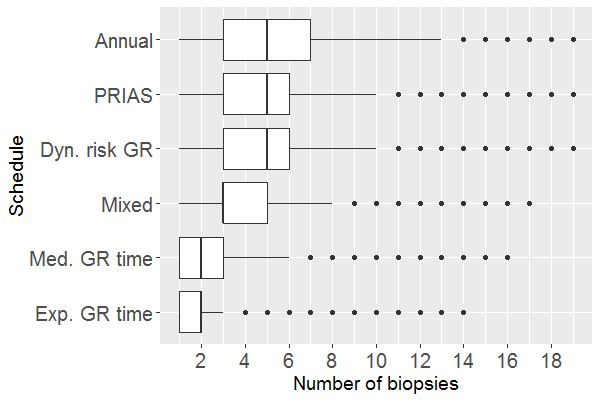
\includegraphics[width=\columnwidth]{images/sim_study/nbBoxPlot_all.png}}
\caption{Boxplot showing variation in number of biopsies conducted by different methods. Patients from all subgroups are considered.}
\label{fig : nbBoxPlot_all}
\end{figure}

\begin{figure}[!htb]
\centerline{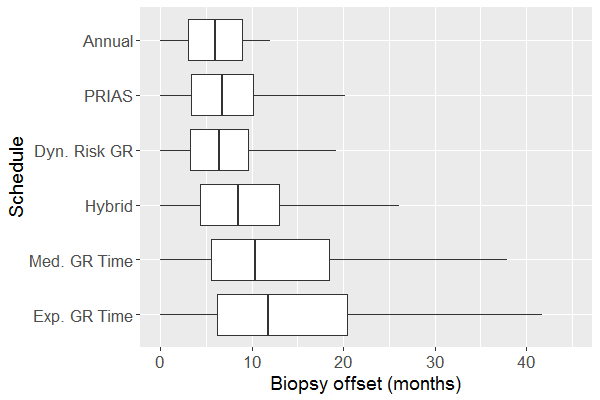
\includegraphics[width=\columnwidth]{images/sim_study/offsetBoxPlot_all.png}}
\caption{Boxplot showing variation in biopsy offset (months) for different methods. Patients from all subgroups are considered.}
\label{fig : offsetBoxPlot_all}
\end{figure}

\begin{figure}[!htb]
\centerline{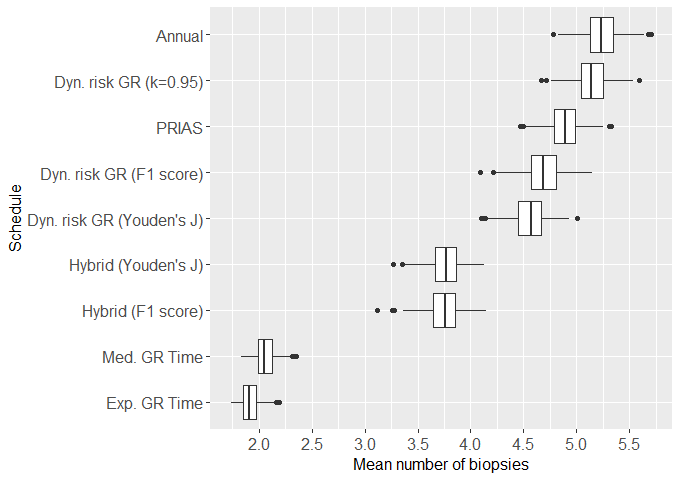
\includegraphics[width=\columnwidth]{images/sim_study/nbMeanBoxPlot_all.png}}
\caption{Boxplot showing variation in estimated mean number of biopsies across the simulations, for different methods. Patients from all subgroups are considered.}
\label{fig : nbMeanBoxPlot_all}
\end{figure}

\begin{figure}[!htb]
\centerline{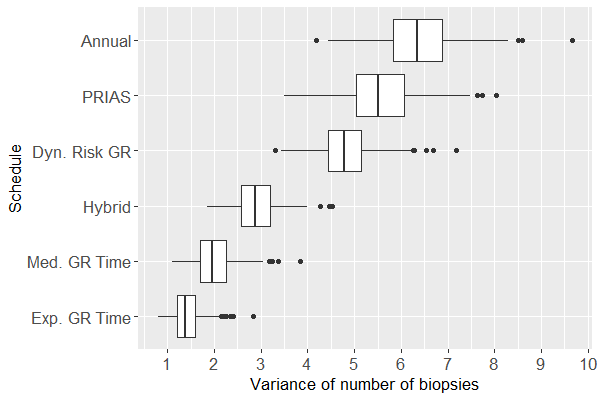
\includegraphics[width=\columnwidth]{images/sim_study/nbVarBoxPlot_all.png}}
\caption{Boxplot showing variation in estimated variance of number of biopsies across the simulations, for different methods. Patients from all subgroups are considered.}
\label{fig : nbVarBoxPlot_all}
\end{figure}

\begin{figure}[!htb]
\centerline{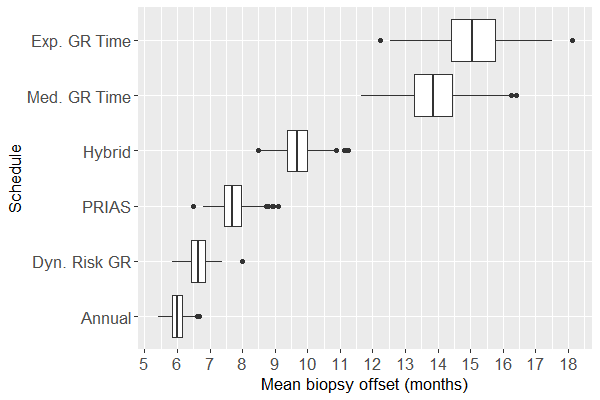
\includegraphics[width=\columnwidth]{images/sim_study/offsetMeanBoxPlot_all.png}}
\caption{Boxplot showing variation in estimated mean of biopsy offset (months) across the simulations, for different methods. Patients from all subgroups are considered.}
\label{fig : offsetMeanBoxPlot_all}
\end{figure}

\begin{figure}[!htb]
\centerline{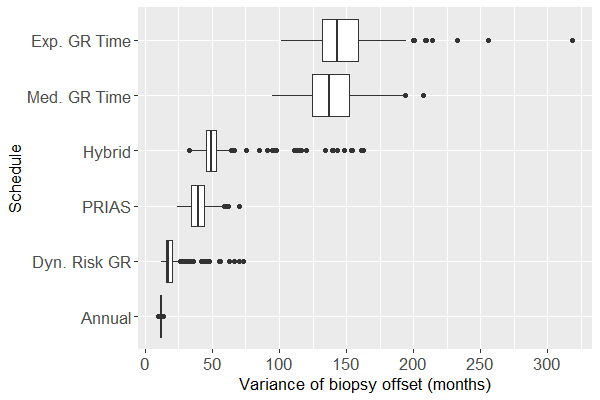
\includegraphics[width=\columnwidth]{images/sim_study/offsetVarBoxPlot_all.png}}
\caption{Boxplot showing variation in estimated variance of biopsy offset (months) across the simulations, for different methods. Patients from all subgroups are considered.}
\label{fig : offsetVarBoxPlot_all}
\end{figure}



